\documentclass[12pt, oneside, openany]{article}
\usepackage[T1]{fontenc}
\usepackage[spanish, es-tabla, es-lcroman]{babel}
\usepackage[utf8]{inputenc}
\usepackage[document]{ragged2e}
\usepackage{tcolorbox}
\tcbuselibrary{theorems}
\usepackage{cancel}
\usepackage{amssymb}
\usepackage{amsmath}
\usepackage{mathrsfs}
\usepackage{wrapfig}
\usepackage{fancyhdr}
\usepackage{colortbl}
\usepackage{longtable}
\usepackage{diagbox}
\usepackage{graphicx}
\usepackage{subcaption}
\usepackage{xcolor}
\usepackage{tikz}
\usetikzlibrary{positioning}
\usepackage{multicol}
\usepackage{multirow}
\usepackage{lastpage}
\usepackage{pdfpages}
\usepackage{listings}
\usepackage{blindtext}
\spanishdecimal{.}
\usepackage[explicit]{titlesec}
\usepackage[colorlinks=true, linkcolor=black, citecolor=black, urlcolor=blue]{hyperref}
\usepackage[a4paper, total={16cm, 24cm}]{geometry}
\pagestyle{fancy}
\lhead{Muñoz Nuñez Ian Emmanuel}
\rhead{Proyecto 8}
\lfoot{Mtra. María Patricia Ventura Nuñez}
\rfoot{CUCEI}
\renewcommand{\headrulewidth}{1pt}
\renewcommand{\footrulewidth}{1pt}

\setlength{\headheight}{14.49998pt}

\definecolor{basicPLD}{RGB}{160, 160, 160}
\definecolor{fondoPLD}{RGB}{40, 40, 40}
\definecolor{commentPLD}{RGB}{0, 240, 170}
\definecolor{keywordsPLD}{RGB}{0, 170, 240}

\lstdefinestyle{SPPSR}{
basicstyle=\ttfamily\small\color{basicPLD},
backgroundcolor=\color{fondoPLD},
commentstyle=\color{commentPLD},
numbers=left,
numberstyle=\ttfamily\small\color{black},
numbersep=5pt,
breaklines=true,
keepspaces=true,
showspaces=false,
showstringspaces=false,
showtabs=false,
xleftmargin=10pt,
emph={PIN, \$DEFINE, FIELD, SEQUENCE, PRESENT, IF, NEXT},
emphstyle=\color{keywordsPLD},
rulesepcolor=\color{magenta},
frame=shadowbox
}
\lstset{style=SPPSR}

\begin{document}

\begin{titlepage}
    \pagenumbering{roman}
    \centering
    {\bfseries\LARGE Universidad de Guadalajara \par}
    \vfill
    {
        \includegraphics[width=0.3\linewidth]{UdG.png}
        \includegraphics[width=0.3\linewidth]{qci.png}
        \par
    }
    \vfill
    {\bfseries\LARGE Seminario de problemas de programación de sistemas reconfigurables \par}
    \vfill
    {\LARGE Diseño e implementación de un contador asíncrono \par}
    \vfill
    {\bfseries\LARGE Nombre: \par}
    \vfill
    {\bfseries\LARGE Muñoz Nuñez Ian Emmanuel \par}
    \vfill
    {\bfseries\LARGE Sección: D01 \par}
    \vfill
    {\bfseries\LARGE Código: 216464457 \par}
    \vfill
    {\bfseries\LARGE Maestra: \par}
    \vfill
    {\bfseries\LARGE María Patricia Ventura Nuñez \par}
    \vfill
    {\bfseries\LARGE Ingeniería Robótica \par}
\end{titlepage}

\pagenumbering{arabic}

\newpage
\section{Objetivo}
{\sffamily\large
    \hspace{0.5cm} Solucionar problemas de diseño utilizando las herramientas aprendidas
    en programación de sistemas reconfigurables.

    \hspace{0.5cm} Simular circuitos digitales en programas de diseño como
    \emph{Proteus\textregistered} e implementarlos físicamente.

    \hspace{0.5cm} Diseño e implementación de un contador asíncrono, por ejemplo,
    contadores de código \emph{BCD's}.
}

\section{Material}
{\sffamily\large
    \renewcommand{\labelitemi}{$\bullet$}
    \begin{itemize}
        \item 2 Protoboard.
        \item Fuente VCC (5V).
        \item Resistencias de $200\Omega$ y $2k\Omega$.
        \item Dip-switch de 4 bits.
        \item 2 Display's de 7 segmentos.
        \item 2 decodificadores \emph{BCD a 7 segmentos}.
        \item 1 \emph{GAL22v10D}.
    \end{itemize}
}

\section{Marco teórico}
\subsection{Secuencias}
{\sffamily\large
    \begin{equation*}
        \begin{split}
            x = 0 & \quad\to\quad 1, 2, 3, 4, 6, 8, 9, 12, 13, 14, 15 \\
            x = 1 & \quad\to\quad 15, 13, 11, 9, 7, 5, 3, 1
        \end{split}
    \end{equation*}
}

\newpage
\subsection{Código desarrollado}
\begin{lstlisting}[
    language=c,
    caption={\sffamily Código desarrollado en \emph{WinCupl}}]
Name     contadorEstados ;
PartNo   00 ;
Date     10/18/2022 ;
Revision 01 ;
Designer ian ;
Company  UdeG ;
Assembly None ;
Location  ;
Device   g22v10 ;

/* CONTADOR X=0 --> 0-12, SI X = 1 --> IMPARES */

/* ENTRADAS */

PIN 1=CK;
PIN 2=X;

/* SALIDAS */
PIN 23=QA;
PIN 22=QB;
PIN 21=QC;
PIN 20=QD;
PIN 19=QE;

FIELD ESTADOS=[QA, QB, QC, QD, QE];
$DEFINE S0 'b' 00000
$DEFINE S1 'b' 00001
$DEFINE S2 'b' 00010
$DEFINE S3 'b' 00011
$DEFINE S4 'b' 00100
$DEFINE S5 'b' 00101
$DEFINE S6 'b' 00110
$DEFINE S7 'b' 00111
$DEFINE S8 'b' 01000
$DEFINE S9 'b' 01001
$DEFINE S11 'b' 10001
$DEFINE S12 'b' 10010
$DEFINE S13 'b' 10011
$DEFINE S14 'b' 10100
$DEFINE S15 'b' 10101

SEQUENCE ESTADOS {
PRESENT S0
IF !X NEXT S1;
IF X NEXT S15;

PRESENT S1
IF !X NEXT S2;
IF X NEXT S15;

PRESENT S2
IF !X NEXT S3;
IF X NEXT S1;

PRESENT S3
IF !X NEXT S4;
IF X NEXT S1;

PRESENT S4
IF !X NEXT S6;
IF X NEXT S1;

PRESENT S5
IF !X NEXT S1;
IF X NEXT S3;

PRESENT S6
IF !X NEXT S8;
IF X NEXT S1;

PRESENT S7
IF !X NEXT S1;
IF X NEXT S5;

PRESENT S8
IF !X NEXT S9;
IF X NEXT S1;

PRESENT S9
IF !X NEXT S12;
IF X NEXT S7;

PRESENT S11
IF !X NEXT S1;
IF X NEXT S9;

PRESENT S12
IF !X NEXT S13;
IF X NEXT S1;

PRESENT S13
IF !X NEXT S14;
IF X NEXT S11;

PRESENT S14
IF !X NEXT S15;
IF X NEXT S1;

PRESENT S15
IF !X NEXT S0;
IF X NEXT S13;
}
\end{lstlisting}

\section{Procedimiento}
{\sffamily\large
    \hspace{0.5cm} Para desarrollar este proyecto primero se hicieron las conexiones entre
    la \emph{GAL}, los decodificadores y los display's, para después hacer el código en
    \emph{WinCupl} y cargarlo a la \emph{GAL}.

    \hspace{0.5cm} Los materiales utilizados para este proyecto son: 1 dip-switch de 4
    bits, 14, resistencias de $220\Omega$ y una de $2k\Omega$, dos decodificadores
    \emph{BCD} a 7 segmentos, 2 display's de 7 segmentos y una \emph{GAL22v10D}.

}

\section{Circuito a implementar}
\subsection{Simulación}
{\sffamily\large
    \hspace{0.5cm} En la siguiente página se muestra el diseño del circuito en
    simulación.

    \newpage
    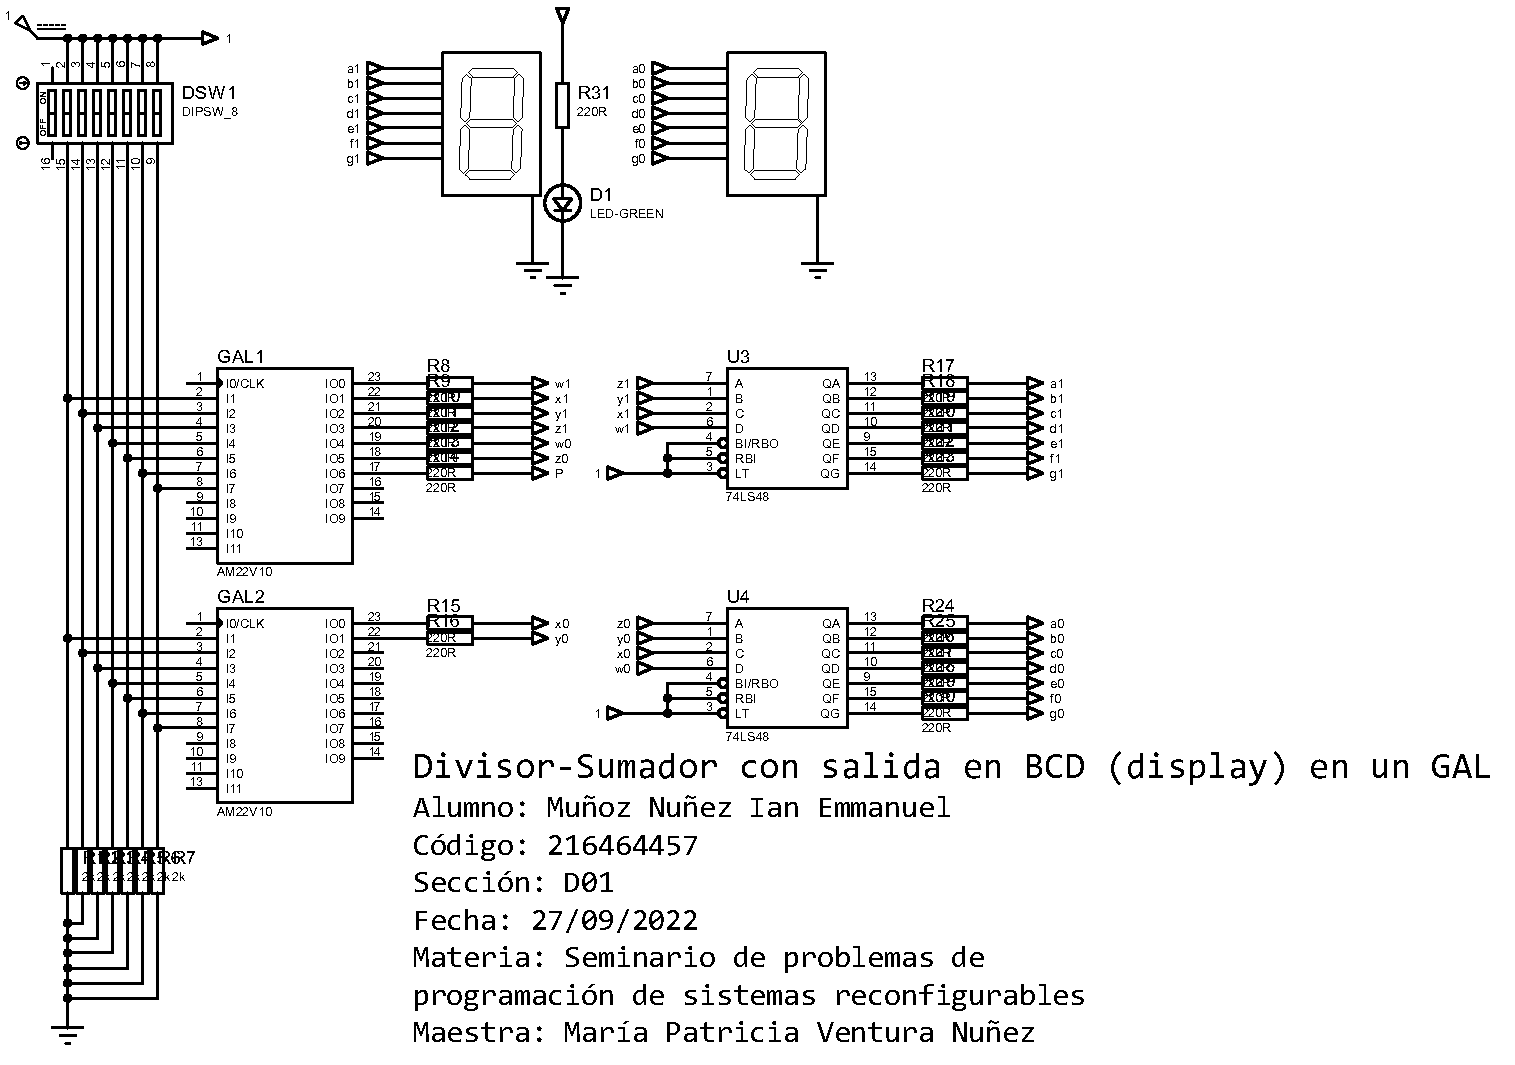
\includepdf[pages={1}]{main.PDF}
}

\subsection{Protoboard}
\begin{figure}[h!]
    \centering

    \begin{subfigure}[tl]{0.45\textwidth}
        \centering
        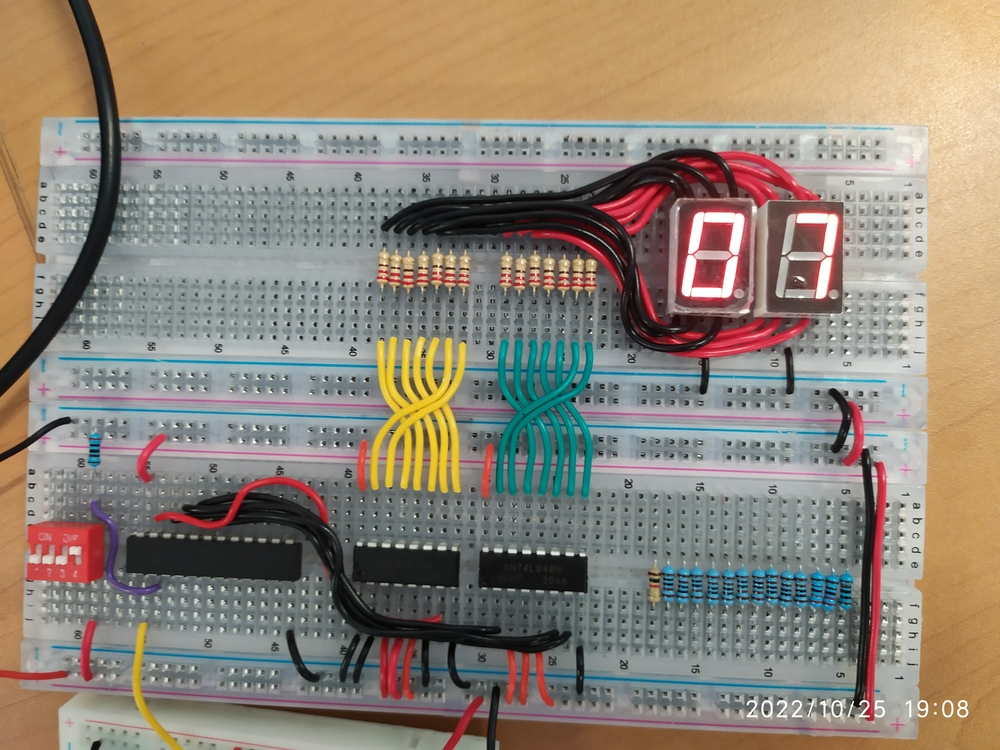
\includegraphics[width=\linewidth]{figs/IMG_20221025_190801.jpg}
    \end{subfigure}
    \begin{subfigure}[tr]{0.45\textwidth}
        \centering
        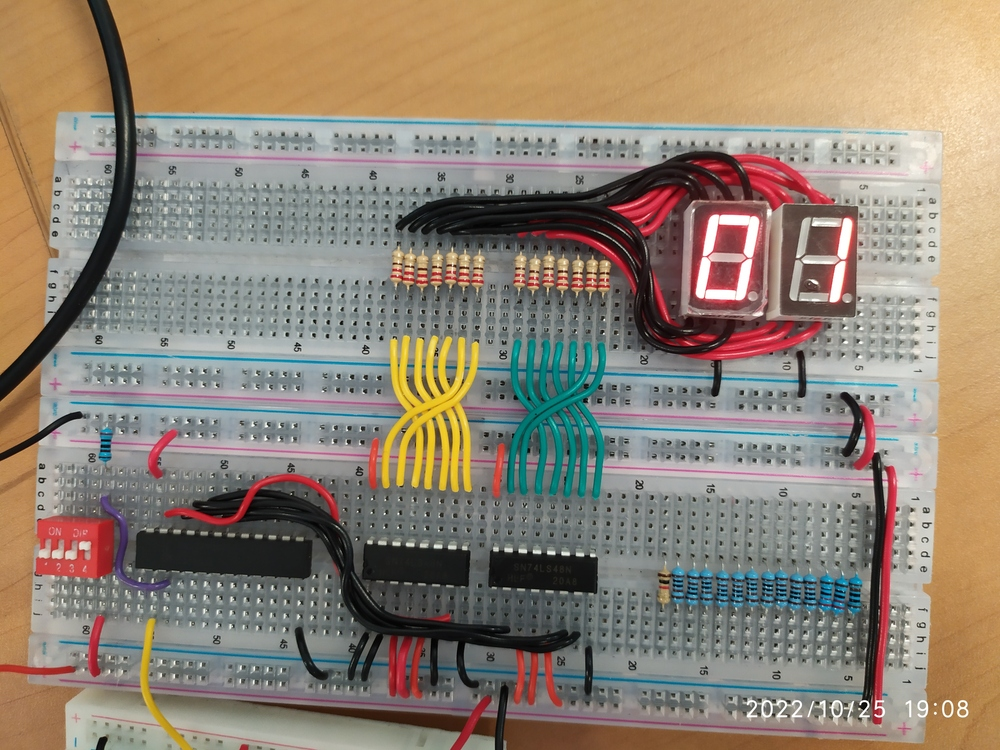
\includegraphics[width=\linewidth]{figs/IMG_20221025_190803.jpg}
    \end{subfigure}
    \begin{subfigure}[bl]{0.45\textwidth}
        \centering
        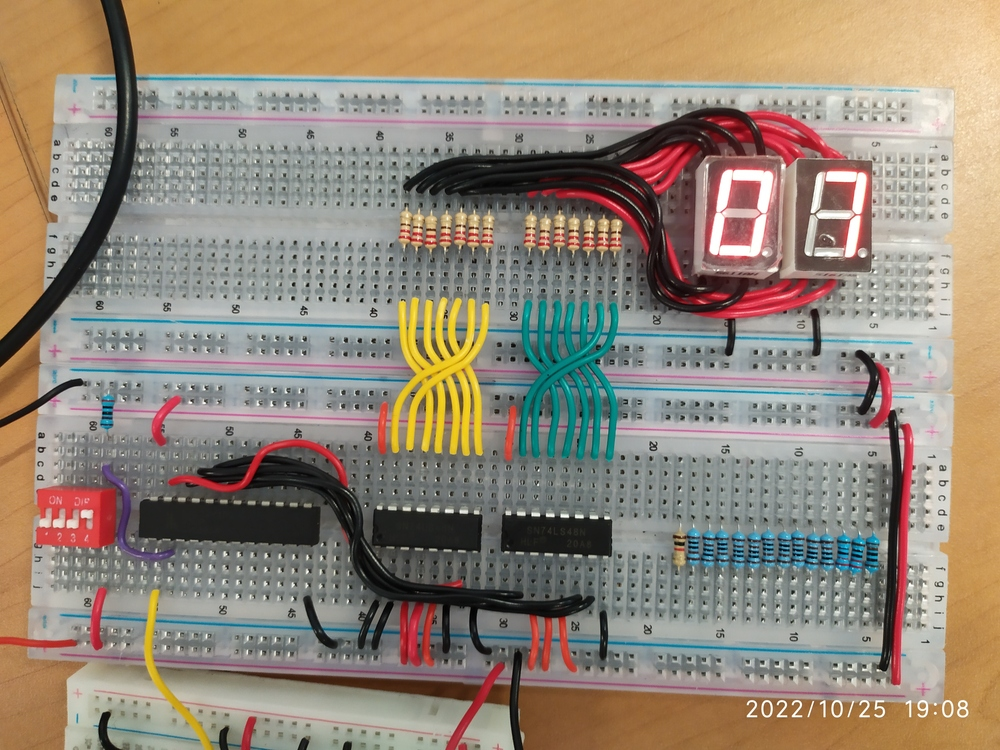
\includegraphics[width=\linewidth]{figs/IMG_20221025_190805.jpg}
    \end{subfigure}
    \begin{subfigure}[br]{0.45\textwidth}
        \centering
        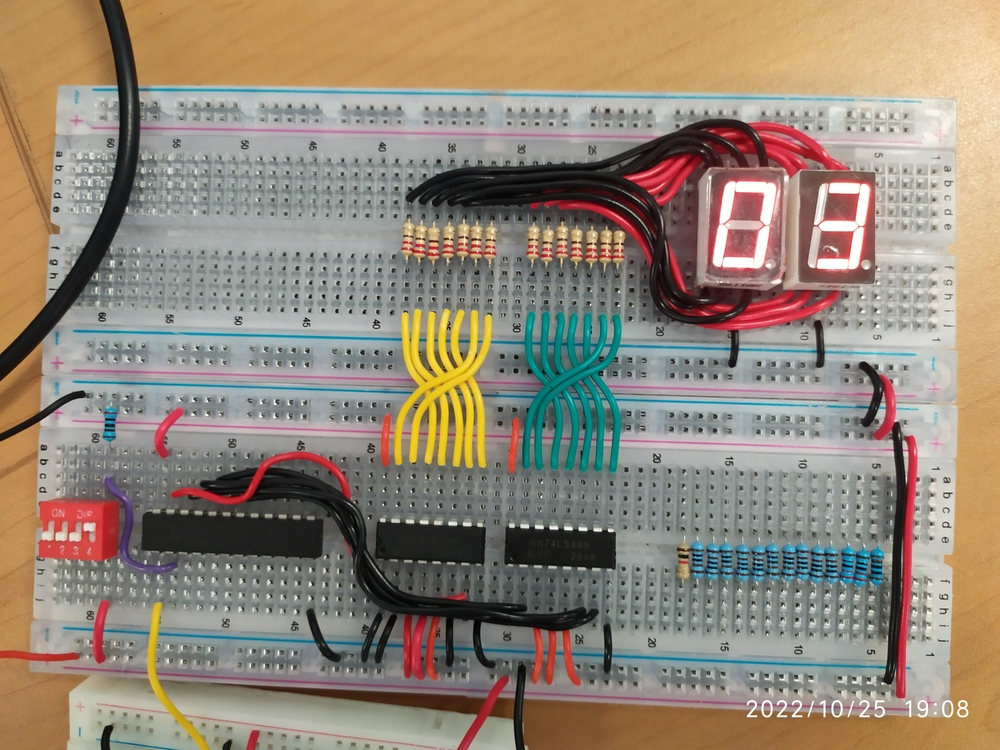
\includegraphics[width=\linewidth]{figs/IMG_20221025_190807.jpg}
    \end{subfigure}

    \caption{\sffamily Circuito en protoboard}
    \label{fig:proto}

\end{figure}

\section{Conclusión}
{\sffamily\large
    \hspace{0.5cm} Usar una \emph{GAL} en lugar de \emph{Flip-Flop's} hace más fáciles
    las cosas, pues no ocupa mucho espacio y todo se realiza a través de software, pero
    al principio es un poco complicado entender como funcionan los estados en la
    \emph{GAL}, pero al final es mejor desarrollar los estados con software que con
    hardware.

}

\end{document}
